% *********************************************************************
% © 2021-2023 Jeremy Sylvestre
%
% Permission is granted to copy, distribute and/or modify this document
% under the terms of the GNU Free Documentation License, Version 1.3 or
% any later version published by the Free Software Foundation; with no
% Invariant Sections, no Front-Cover Texts, and no Back-Cover Texts. A
% copy of the license is included in the appendix entitled “GNU Free
% Documentation License” that appears in the output document of this
% PreTeXt source code. All trademarks™ are the registered® marks of
% their respective owners.
%
% *********************************************************************

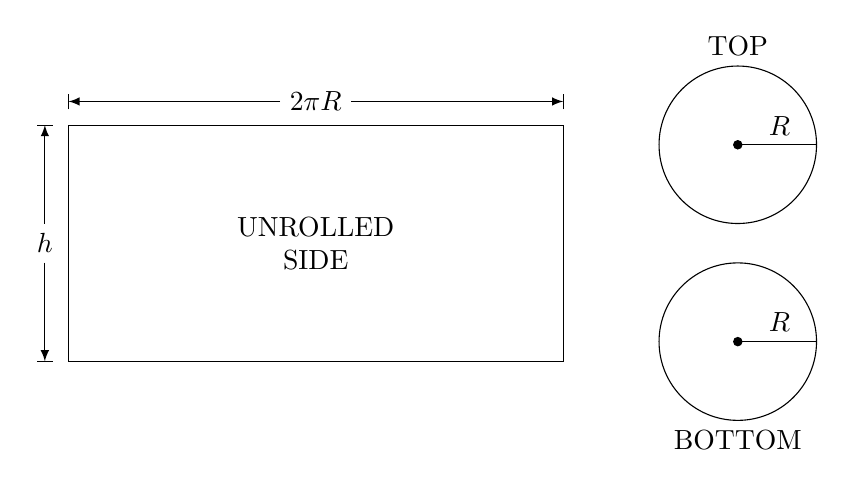
\begin{tikzpicture}[
	closedpt/.style={circle,draw,fill,inner sep=0pt,minimum size=3pt}
]

	\draw (-2.2,3) -- (-2.4,3);
	\draw (-2.2,0) -- (-2.4,0);
	\node at (-2.3,1.5) (h) {$h$};
	\draw[-latex] (h) -- (-2.3,3);
	\draw[-latex] (h) -- (-2.3,0);

	\draw (-2,3.2) -- (-2,3.4);
	\draw (4.283,3.2) -- (4.283,3.4);
	\node at (1.14,3.3) (C) {$2 \pi R$};
	\draw[-latex] (C) -- (-2,3.3);
	\draw[-latex] (C) -- (4.283,3.3);

	\draw (-2,3) rectangle (4.283,0);

	\draw (6.5,0.25) circle (1cm);
	\node[closedpt] at (6.5,0.25) (c) {};
	\draw[thin] (c) -- node[above] {$R$} (7.5,0.25);

	\draw (6.5,2.75) circle (1cm);
	\node[closedpt] at (6.5,2.75) (c) {};
	\draw[thin] (c) -- node[above] {$R$} (7.5,2.75);

	\node[align=center] at (1.14,1.5) {UNROLLED \\ SIDE};
	\node at (6.5,4) {TOP};
	\node at (6.5,-1) {BOTTOM};

\end{tikzpicture}
